%\documentclass[aps,prl,twocolumn,nobibnotes]{revtex4}
\documentclass[aps,showpacs,twocolumn,nobibnotes]{revtex4}
%\documentclass[aps,preprint,showpacs,nobibnotes]{revtex4}
%\documentclass[aps,preprint,nobibnotes]{revtex}
\usepackage{graphics,graphicx,amsfonts,amsmath,amsbsy,amssymb,color}
\usepackage{bm}
%\usepackage{epic}
%\usepackage{mciteplus}
\usepackage{subfigure}
\usepackage{vector}  % Allows "\bvec{}" and "\buvec{}" for "blackboard" style bold vectors in maths
\newcommand{\D}[1] {D_{\bf #1}}
\def \beq {\begin{eqnarray}}
\def \eeq {\end{eqnarray}}
\def \Schrodinger {{Schr\"{o}dinger }}
\def \Di {{D_{\bfi}}}
\def \Dj {{D_{\bfj}}}
\newcommand {\adag}[1] {{a_{#1}^\dagger}}
\def \bfj {{\bf j}}
\def \bfi {{\bf i}}
\def \rone {{\bvec{r}_1}}
\def \rtwo {{\bvec{r}_2}}
\def \mEh {{\textrm{mE}_{\textrm{h}}}}
\def \Eh {{\textrm{E}_{\textrm{h}}}}
\def \nadd {{n_a}}
\newcommand{\braket}[3] {{\langle #1 | #2 | #3 \rangle}}
\newcommand{\brket}[2] {{\langle #1 | #2 \rangle}}
\newcommand{\bra}{\ensuremath{\langle}}
\newcommand{\ket}{\ensuremath{\rangle}}
%\def \ham {{\bf H}}
\def \ham {{\hat{H}}}
%\def \Sz {{\hat{\textrm{S}_{\textrm{z}}}}}
\def \Sz {{\hat{S}_z}}
\newcommand{\rff}[1]{{Eq.~\eqref{#1}}}
\def \Pgen {{P_{\textrm{gen}}}}
\def \Carb {{\textrm{C}_{\textrm{2}}}}
\def \Hij {{H_{\bvec{i}\bvec{j}}}}
\def \Kii {{K_{\bvec{i}\bvec{i}}}}
\def \Kij {{K_{\bvec{i}\bvec{j}}}}

\begin{document}
\title{Spectral functions of extended systems via quantum embedding}
\author{George~H.~Booth}
%\email{ghb24@cam.ac.uk}
\author{Garnet~Kin-Lic~Chan}  
\affiliation{Department of Chemistry, Frick Laboratory, Princeton University, Princeton, New Jersey 08544, USA}

\begin{abstract}
In a previous publication [PRL {\bf 109} 186404 (2012)], the ground-state density matrix embedding theory (DMET) was introduced for the seamless embedding of
strongly entangled wavefunctions within an extended environment. 
%With similarities 
%to the dynamical mean-field method, a set of local sites are self-consistently correlated, but with an analytically constructable bath describing the
%coupling to the rest of the extended system. 
Despite many formal advantages in the analytic embedding, the method was restricted to static, ground-state properties.
Here, we generalise the concept of quantum embedding to introduce a frequency dependence and demonstrate accurate spectral functions at a tiny
computational cost. Through this quantum embedding of a local spectral function within a one-electron response over the whole system, 
a coupling is introduced through a small set of 
analytically constructed, but now frequency-dependent bath states. In contrast to dynamical mean-field theory, the resultant 
spectral functions are directly obtained on the real-frequency axis, with no bath discretization error, and allow for straightforward generalization both 
to impurity clusters and arbitrary electron perturbation operators. We demonstrate
the application of this method to the Hubbard model, where both the the Kondo resonances and metal-insulator transitions are well reproduced, as well as 
demonstrating two-electron spectra. We believe that for the low-energy excitations, these results represent some of the most accurate 
zero temperature, thermodynamic limit spectral functions for the Hubbard model to date. This vastly extends the scope and applicability 
of the DMET method in condensed matter problems as a computationally tractible route to correlated spectral functions of extended systems.
\end{abstract}
\date{\today}
\maketitle

Dynamic correlation functions are directly probed in most spectroscopic methods, as well as other techniques such as scanning tunnelling microscopy (STM), 
and correspond to many of the important transport, optical and wider electronic structure properties of materials. 
As such, their accurate computational prediction is highly sought after within the materials science community. 
However, few robust approaches exist for strongly correlated problems\cite{Gali2013}. The difficulty is in simultaneously requiring both an accurate 
treatment of the electron correlations beyond mean-field band theory for the ground state {\em and} excitation spectrum, as well as modelling 
a system of sufficient size to mimic the thermodynamic limit of bulk properties and not suffer spurious finite size effects. 
However in general, it is only mean-field electronic structure methods which are computationally cheap enough to access the required system
sizes, and so there is a pressing need for methods with mean-field scaling, which can account for the excitation spectrum in strongly correlated 
and entangled systems.

A general, zero-temperature dynamic correlation function can be defined in the frequency domain as
\begin{equation}
    G(\omega) = \langle \Psi_0 | A^{\dagger} \frac{1}{\omega-(H-E_0)+i \eta} V | \Psi_0 \rangle , \label{eqn:intCorrFunc}
\end{equation}
with the one- and two-particle Greens functions defined with $V$ and $A$ being single annihilation/creation operators or neutral excitation
operators respectively, with appropriate time-ordering of the operators. Spectral quantities are then defined as $A(\omega)=-\frac{1}{\pi}\Im[G(\omega)]$,
where the spectral broadening is given by the small imaginary component of the energy, $\eta$, which regularizes the correlation function. The single particle
density of states is given by the spectral representation of the one-particle Greens function, experimentally measured within STM and (angle-resolved) photoemission
spectroscopy. However, other spectral functions are also highly sought after, such as the two-hole propagator, probed with Auger spectroscopy\cite{Mona2013}, or the two-electron
Greens function, a key descriptor in Raman spectroscopy, and in the mechanism of high-temperature superconductivity\cite{Millis2012,Millis2013}.

One such method which has proven very successful in obtaining strongly correlated spectral functions is the dynamical mean-field theory (DMFT). In DMFT, the central variable is the
local, one-particle Greens function, which is self-consistently embedded within a non-interacting or mean-field Greens function over the system. This impurity problem is then solved via
an `impurity solver', such as continuous-time quantum Monte Carlo (CT-QMC). However, there are some formal drawbacks of the DMFT formulation. If CT-QMC is used as an impurity solver, then
the spectral functions are obtained only on the imaginary frequency axis, requiring unstable analytic continuation onto the real frequency axis, which can wash out the subtle features of the spectra. Alternative solvers such as exact diagonalization
suffer from bath discretization error in the spectra due to the representation of the coupling to the continuum (at all frequencies) by a finite number of bath sites. In addition, since DMFT
is formulated around the one-particle Greens function, alternative spectra such as the two-particle Greens function and optical spectra are not straightforward to obtain, formally 
requiring expensive vertex corrections to compute\cite{Millis2012}.

Here, we aim to circumvent these issues, by generalizing and extending the idea of quantum embedding of {\em states}, as introduced in Ref.~\onlinecite{Chan2012}. 

Size of bath independent of the size of the underlying lattice. Only a function of the impurity cluster size and the perturbation, while still exact in the non-interacting limits.

Coupling only within the bandwidth of the 1 electron bath
Plotted within the bandwidth of the 1 electron 

1 electron response operator is partitioned into the schmidt basis, such that a block acts purely in the schmidt basis of the ground state embedded space, 

Schmidt decompose the action of the non-interacting operator, into that acting on the space of the impurity+bath ground state system, and that acting on the rest of the environment orbitals.

Cost of any frequency point not more than a minute on a single processor core.

DD results using reoptimized ground state.

Within the 1 electron response function bandwidth

Doped Spectral functions in 1D with DMRG: PRL (2004) 256401, 92

ED can only treat small clusters, and therefore the relatively small numbers of poles that are unable to be resolved into the spectral functions of the extended system. Perturbation theory, 
correlation only treated to low order, and will 
lose accuracy as you tend towards to opposite coupling limit to the zeroth order solution (PRL 84 522 1999), and QMC is formulated in imaginary time, and therefore the maximum entropy is needed,
washes out the subtle feature of the spectrum.


Gap measured from Single-particle spectrum as the difference between the energy of the lowest electron peak and that of the highest hole peak in the single-particle DoS.

Continuous Weiss field approximated by a finite number of bath sites - require convergence with respect to this parameter, while computational effort will generally increase exponenetially wrt this number.

Can be computed via the 1-particle or 2-particle greens function

Possible to reoptimize the ground state in the space of V*|0>, but this was found not to materially change results, and so is not performed from the results presented here.


\emph{Method.-} Within the analytic quantum embedding formalism introduced for the ground state with the DMET method (see Ref.~\onlinecite{Chan2012,Chan2013} for details), the coupling between the 
correlated `impurity' sites, $|\alpha \rangle$, and the rest of the
system is represented via the component of the Schmidt basis of a one-electron function over the `environment' space external to the impurity. This space is denoted the 
ground-state {\em bath}, $|\beta \rangle$, and analytically spans the exact entanglement of the impurity space to its environment, as defined by the original one-electron function
over the entire extended lattice. The interacting Hamiltonian is then projected into this space, which is now independent of the total number of sites, and solved to return a wavefunction 
in the space of $\{ |\alpha \rangle \} \otimes \{ |\beta \rangle \} \otimes \rm{det[ext]}$, where det[ext] represents the space of the one-electron function which is uncoupled to the impurities
after the Schmidt decomposition. From the ground-state DMET calculation, along with the bath space, a self-consistency procedure returns a one-electron interaction potential, $u$ which
describes some of the longer-ranged correlation effects, and determines the effective number of electrons in the impurity cluster.

We now generalize this procedure for embedding within a one-electron linear response vector, in order to create an analogous set of frequency-dependent bath states
into which the impurity problem can be projected. In this letter, we restrict ourselves to consider one- and two-electron Greens functions for simplicity, 
while other dynamic correlation functions can be obtained analogously.

The is one-electron wavefunction is defined as,
\begin{equation}
    |\phi^{(1)}(\omega) \rangle = \frac{{\hat V} }{\omega-(h-e_0)+i\eta}|\phi^{(0)}\rangle  , \label{nonintGF}
\end{equation}
where the desired zero-temperature Greens function is then defined



(Due to the special properties of the Schmidt decomposition of a single determinant, the ground-state bath in 


%+++++++++++++++++++++++++++++++++++++++++++++++++++++++
%   1D HUBBARD MODEL PLOTS vs. CDMFT
%+++++++++++++++++++++++++++++++++++++++++++++++++++++++
\begin{figure}
\begin{center}
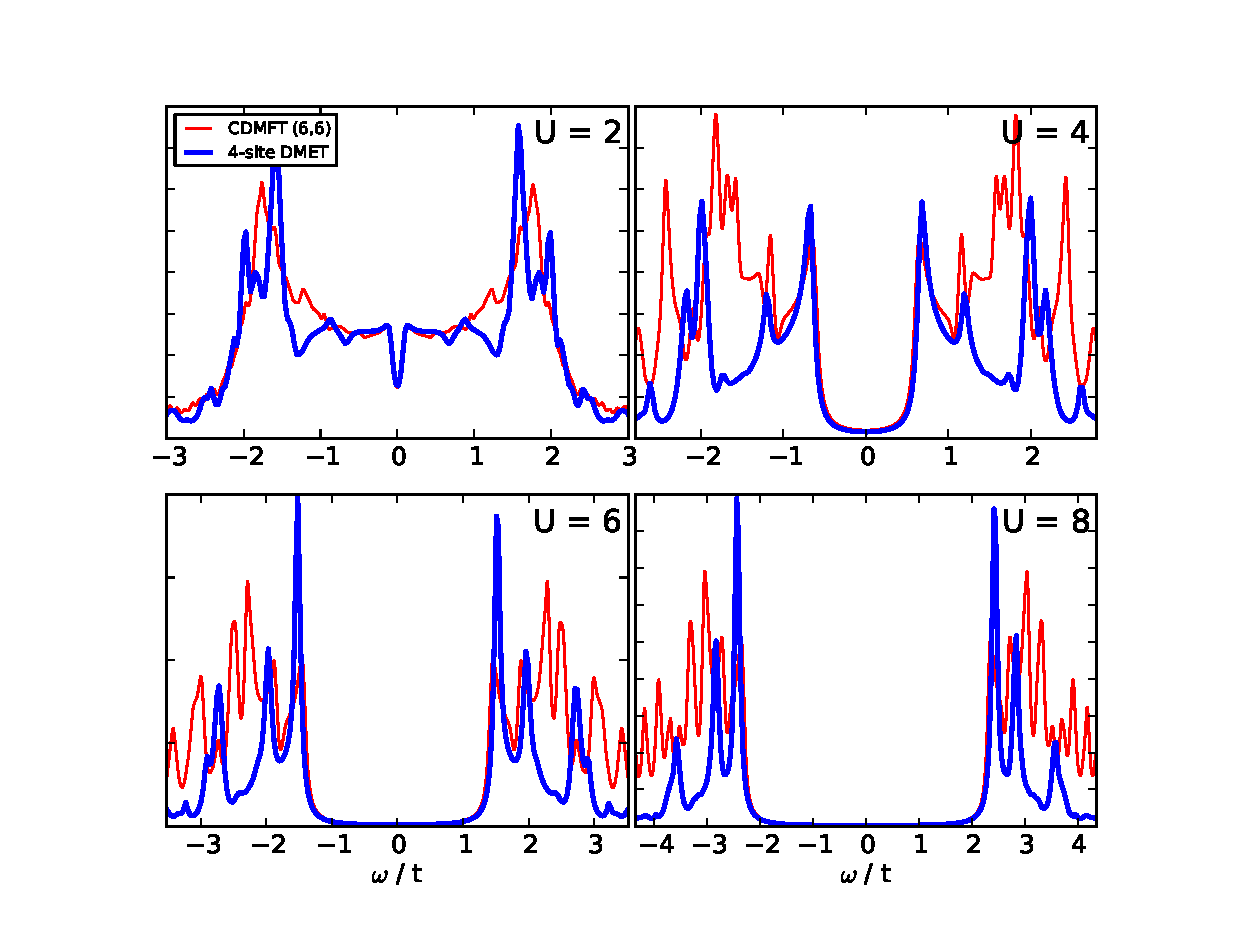
\includegraphics[scale=0.475]{Plots/1D_Spectra/1D_Hub_Spectra.eps}
\end{center}
\caption{Comparison of the local density of states from a four impurity cluster DMET calculation with a
(six impurity, six bath) CDMFT calculation for the half-filled 1D Hubbard model.}
\label{1D_DOS}
\end{figure}

%+++++++++++++++++++++++++++++++++++++++++++++++++++++++
%   1D HUBBARD SPECTRAL GAP 
%+++++++++++++++++++++++++++++++++++++++++++++++++++++++
\begin{figure}
\begin{center}
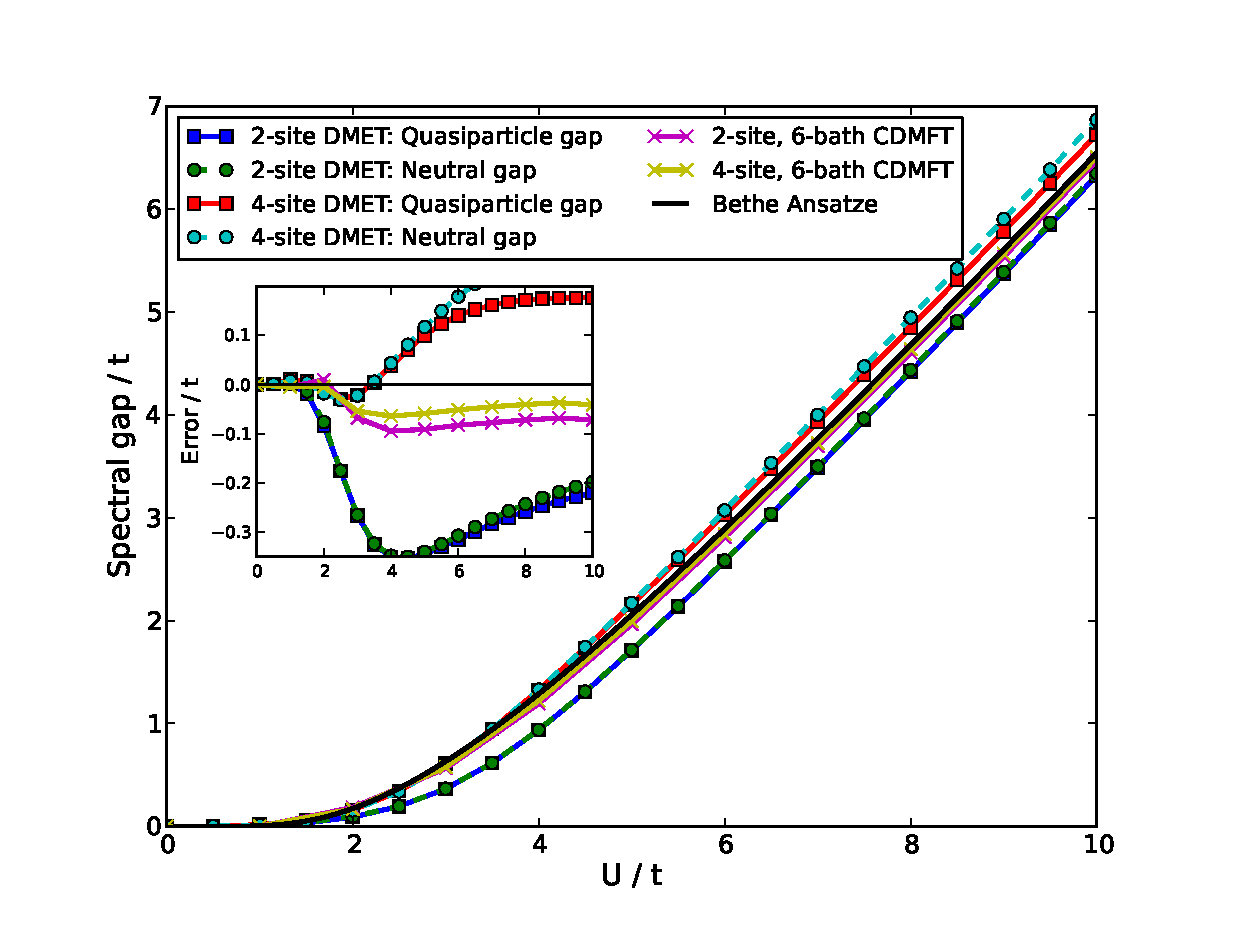
\includegraphics[scale=0.475]{Plots/1D_Gap/Hubbard_Gap.eps}
\end{center}
\caption{Spectral gap from the 1-particle and 2-particle greens functions compared to analytic results
from the Bethe Ansatze\cite{Ovchinni1970}.}
\label{1D_GAP}
\end{figure}


%+++++++++++++++++++++++++++++++++++++++++++++++++++++++
%   2D HUBBARD PLOTS 
%+++++++++++++++++++++++++++++++++++++++++++++++++++++++
\begin{figure}
\begin{center}
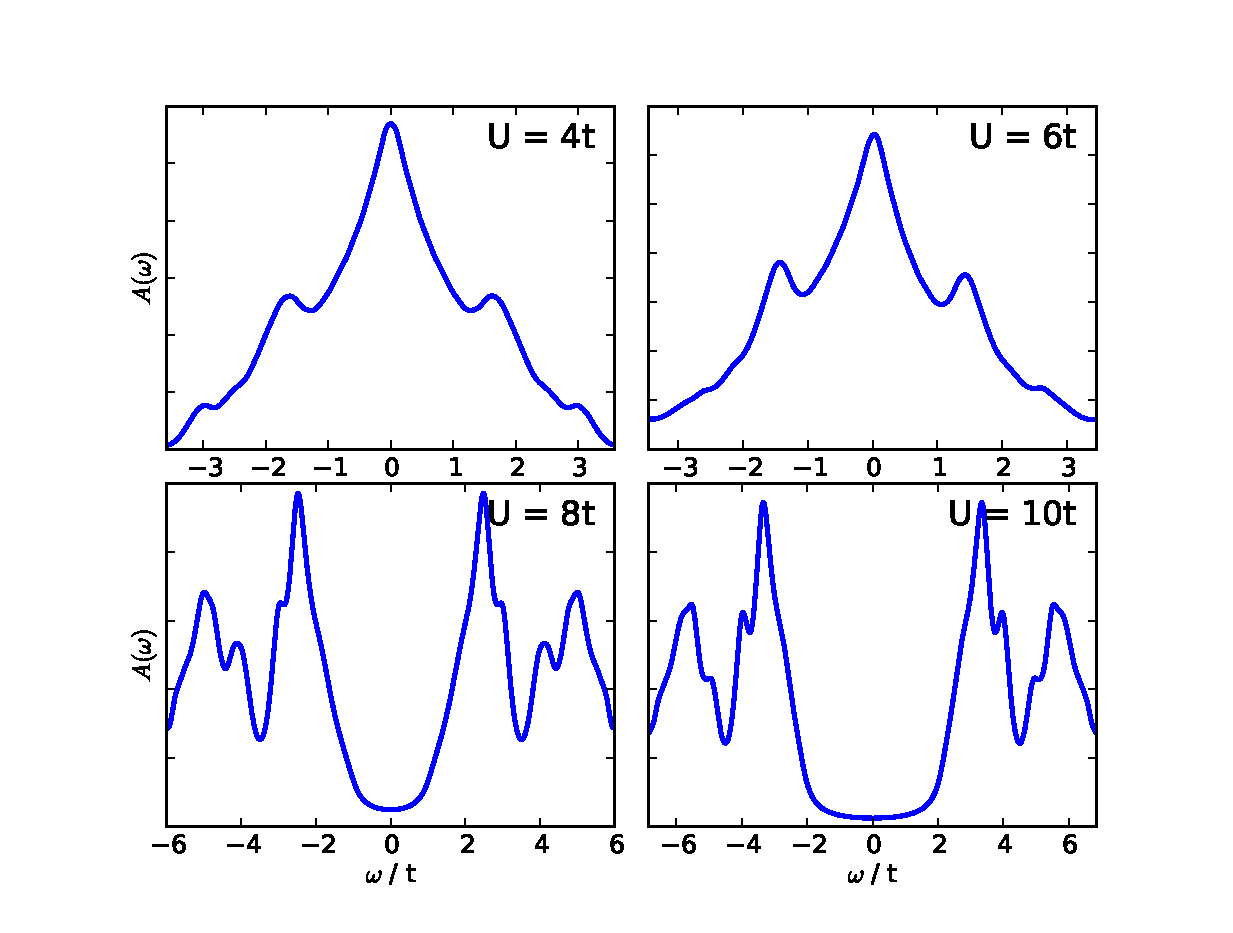
\includegraphics[scale=0.475]{Plots/2D_Spectra/2DHub_Spectra.eps}
\end{center}
\caption{Local density of states of the half-filled 2D hubbard model from a four impurity DMET calculation.}
\label{2D_DOS}
\end{figure}


%+++++++++++++++++++++++++++++++++++++++++++++++++++++++
%   2D DOPED HUBBARD PLOTS 
%+++++++++++++++++++++++++++++++++++++++++++++++++++++++
\begin{figure}
\begin{center}
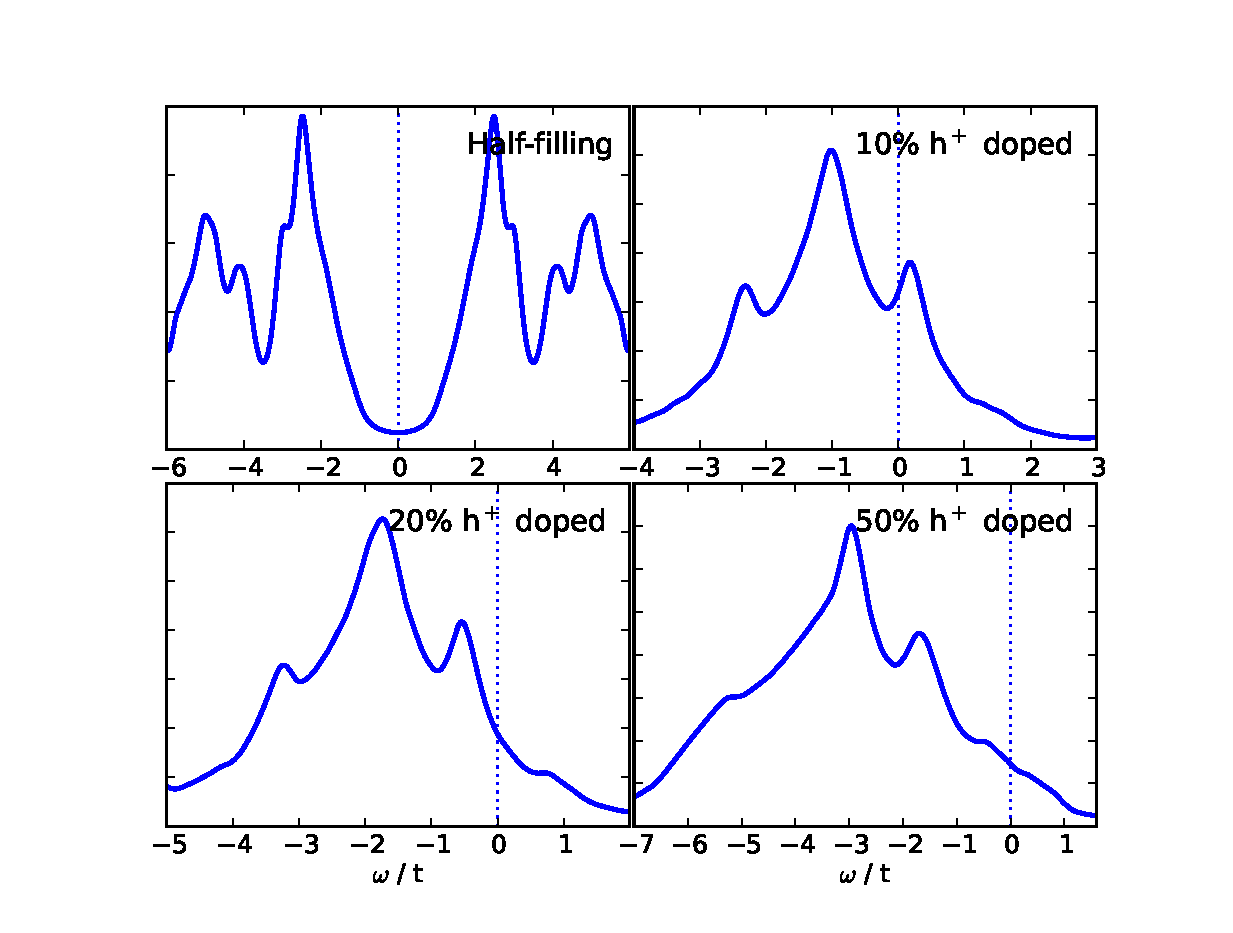
\includegraphics[scale=0.475]{Plots/Doping/2D/nImp4/U8/LargerBroadening/2DHub_Doping.eps}
\end{center}
\caption{Local density of states of the hole doped 2D hubbard model from a four impurity DMET calculation with $U = 8t$.}
\label{2D_Doped}
\end{figure}

%+++++++++++++++++++++++++++++++++++++++++++++++++++++++
%   DD response 
%+++++++++++++++++++++++++++++++++++++++++++++++++++++++
\begin{figure}
\begin{center}
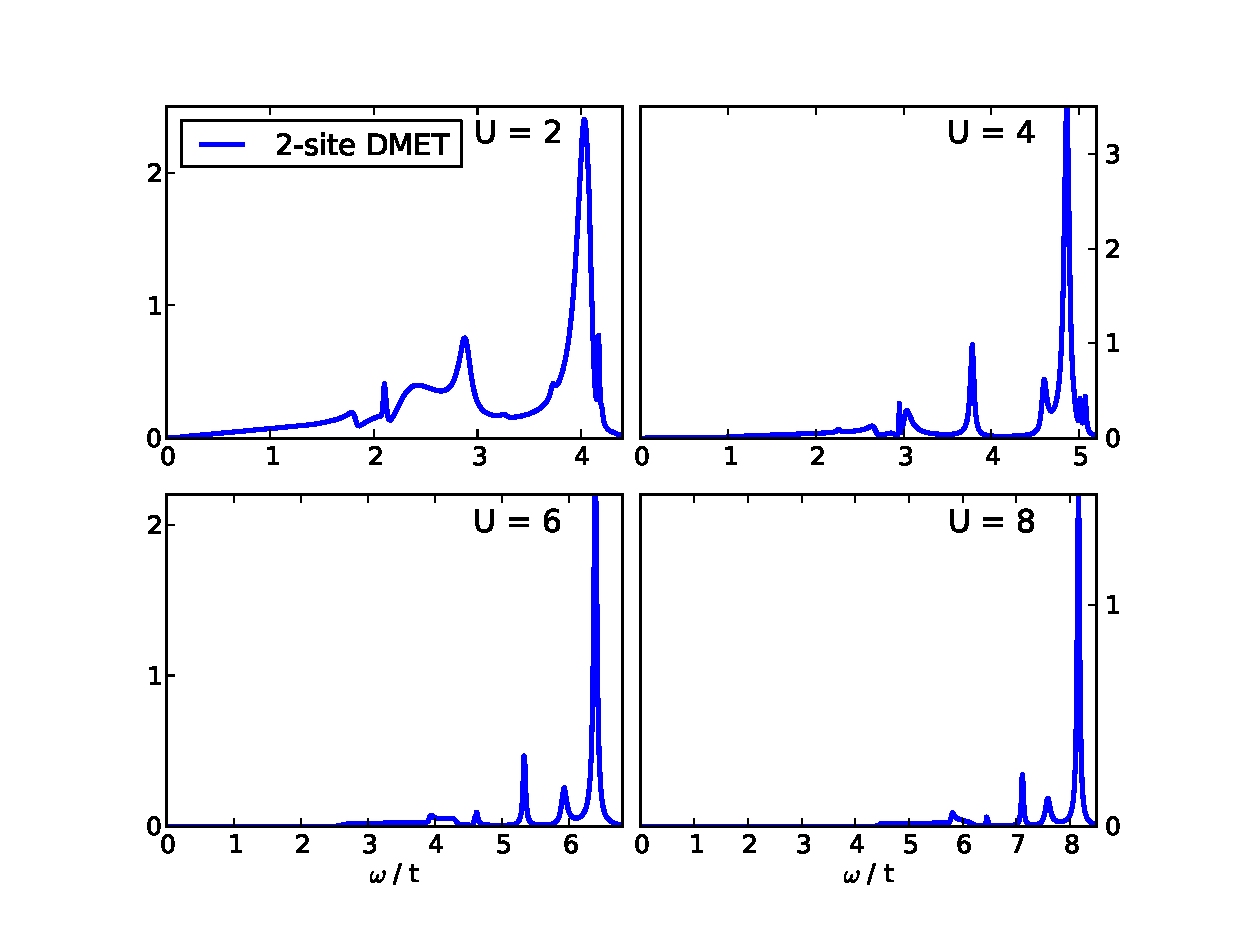
\includegraphics[scale=0.475]{Plots/1D_DD/1D_Hub_DD.eps}
\end{center}
\caption{Two impurity DMET calculation of the local density-density response function for the half-filled 1D hubbard model via construction of the 2-particle greens function.
The spectral gap is used in the data plotted in Fig.~\ref{1D_GAP}}
\label{1D_DD}
\end{figure}



\bibliography{SpectralDMETBib}

\end{document}
